\chapter{Latex Ticks}

\section{Figure Overlap On The Plain Text}

\begin{frame}

\lstset{
  basicstyle=\fontsize{8}{10}\selectfont\ttfamily
}
\begin{lstlisting}[language=java]
class MakeFramee extends JFrame {
	
	private Container container = null;
	public JLabel imgLabel = null;
	private ImageIcon icon = null;
	private Image img = null;

	MakeFramee(){
		decorateFrame();
	}
	
	public void decorateFrame() {
		
		container = this.getContentPane();
		container.setLayout(null);
		
		this.setDefaultCloseOperation(EXIT_ON_CLOSE);

		//----- Set Image Label
		icon = new ImageIcon(getClass().getResource("user_Icon.png"));
		img = icon.getImage();
		img = img.getScaledInstance(100, 100, Image.SCALE_SMOOTH); // Resize Image
		icon = new ImageIcon(img);				// Re-assign image to icon
		imgLabel = new JLabel(icon);			// Instantiate image Label
		imgLabel.setBounds(100,100,200,200);
		imgLabel.setOpaque(true);
		imgLabel.setBackground(Color.cyan);
		container.add(imgLabel);				// Add image to container
	}
}

\end{lstlisting}

\begin{tikzpicture}[remember picture,overlay]
	\node[anchor=north east] at ([xshift=-1cm,yshift=-7cm]current page.north east) {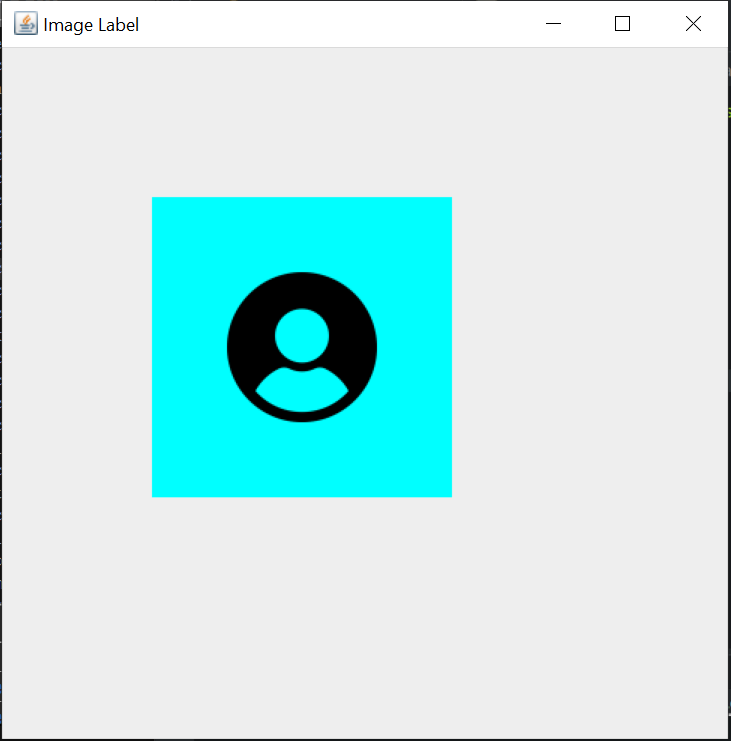
\includegraphics[width=7cm]{Figures/imgLabel.PNG}};
\end{tikzpicture}

\end{frame}



%--------------- Efficient Control Over the figure ----------------
\newpage
\section{More Control over the Figure }
\begin{frame}

\AddToShipoutPictureFG*{ % Add figure to foreground of current page
  \put(\LenToUnit{13cm},\LenToUnit{7cm}){% Adjust the coordinates as needed
    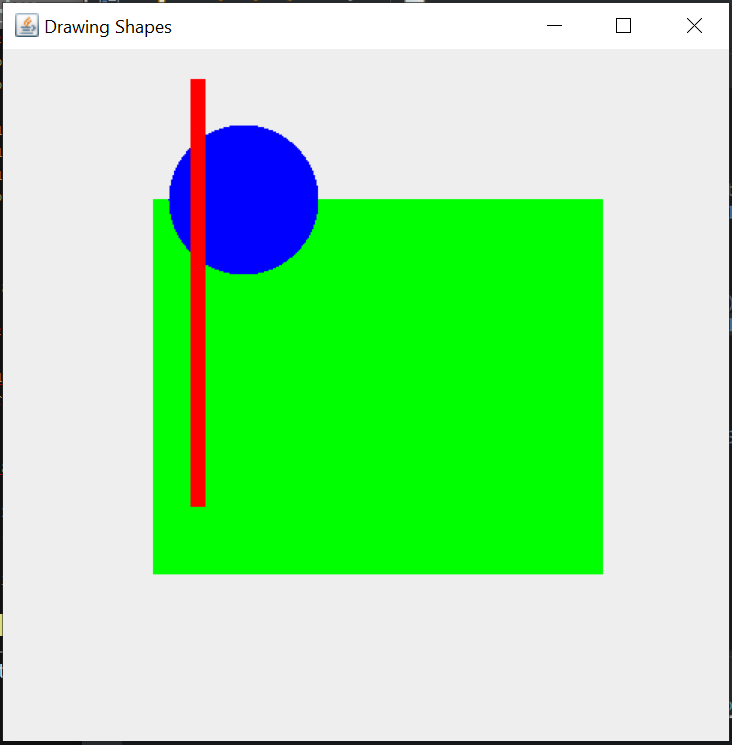
\includegraphics[width=7cm]{Figures/drawShape.PNG}
  }
}

\lstset{
  basicstyle=\fontsize{8}{10}\selectfont\ttfamily
}
\begin{lstlisting}[language=java]
DrawingPanel() {
		
		this.setTitle("Drawing Shapes");
		this.setSize(500,500);
		this.setLocationRelativeTo(null);
		this.setDefaultCloseOperation(EXIT_ON_CLOSE);
		
		JPanel drawintPanel = new JPanel() {
			public void paintComponent(Graphics g) {
				Graphics2D g2 = (Graphics2D) g;
				
				//Rectangle2D.Double(x,y,width,height);
				Shape rect = new Rectangle2D.Double(100,100,300,250);
				g2.setColor(Color.GREEN);
				g2.fill(rect);
				
				// Ellipse2D.Double(x,y,width,height);
				Shape circle = new Ellipse2D.Double(110,50,100,100);
				g2.setColor(Color.blue);
				g2.fill(circle);
				
				// Draw line form (x1,y2) to (x2,y2)
				Shape line = new Line2D.Double(130,25,130,300);
				g2.setStroke(new BasicStroke(10));
				g2.setColor(Color.red);
				g2.draw(line);	
			}
		};
		
		this.getContentPane().add(drawintPanel);
		this.setVisible(true);
	}
}

public class DrawingApp {
	public static void main(String[] args) {
		DrawingPanel frame = new DrawingPanel();
	}
}

\end{lstlisting}


\end{frame}
